\documentclass[11pt,a4paper]{article}

\usepackage[utf8]{inputenc}
\usepackage[T1]{fontenc}
\usepackage{amsmath,amssymb,amsfonts}
\usepackage{geometry}
\usepackage{cite}
\usepackage{booktabs}
\usepackage{graphicx}
\usepackage{caption}

\geometry{margin=1in}

\title{G-quAI \\ \large Hardware-Native Quantum Convolutional Neural Networks on QuEra Aquila for Medical Image Classification}
\author{Team G-quAI, University of Coimbra}
\date{\today}

\begin{document}

\maketitle

\begin{abstract}
\textbf{G-quAI} is a research initiative based at the University of Coimbra dedicated to the early detection of colorectal cancer from high-resolution gastrointestinal medical imaging using Quantum Artificial Intelligence. Classical deep learning for such high-variance medical imaging requires massive computational clusters. We aim to leverage hardware-native quantum phenomena to reduce this computational overhead while increasing diagnostic sensitivity. While our ultimate goal targets colorectal cancer, this specific experimental proposal serves as a crucial hardware proof-of-concept utilizing the \textbf{BreastMNIST} dataset. BreastMNIST contains highly noisy, low-resolution ultrasound images with a manageable low sample count, making it an ideal, iterative testbed for quantifying the diagnostic advantage of quantum physics prior to scaling to high-resolution endoscopic datasets. For this phase, we are requesting resources to run our \textit{Digital} encoding experiments on the QuEra Aquila system.
\end{abstract}

\section*{1. Motivation: Why the Quantum Domain?}
Our work is grounded in the architectural advantages of Digital-Analog Quantum Kernels (DAQKs) as proposed by Simen et al. \cite{daqcnn2024}. The transition to the quantum domain for medical image classification is motivated by three primary factors:
\begin{enumerate}
    \item \textbf{High-Dimensional Feature Mapping:} Quantum kernels naturally map classical data into a high-dimensional Hilbert space where classes that are non-linearly separable in the original space may become linearly separable.
    \item \textbf{Complexity via Native Interactions:} Unlike classical CNNs where filters are trained via backpropagation, DAQCNNs leverage the fixed, native ``complexity'' of Rydberg atom interactions to extract intricate spatial correlations and multipartite entanglement dynamics that classical filters may fail to capture.
    \item \textbf{Massive Parameter Efficiency:} DAQCNNs have demonstrated the ability to outperform classical state-of-the-art models while using significantly fewer trainable parameters (often by orders of magnitude), directly addressing the energy and computational bottlenecks of modern medical AI.
\end{enumerate}

\section*{2. Methodology: ZZ-AQCNN \& Encoding Schemes}
Our approach, the \textbf{ZZ-AQCNN}, enhances the DAQCNN framework by measuring both 1-body ($\langle \sigma_Z^{(i)} \rangle$) and 2-body ($\langle \sigma_Z^{(i)} \sigma_Z^{(j)} \rangle$) correlators. For a 9-qubit kernel, this expands our feature space to 45 densely correlated features. 

We utilize two primary encoding schemes:
\begin{enumerate}
    \item \textbf{Digital Encoding:} Data is encoded in the initial state via $RY(x_i)$ and $H$ gates at $t=0$:
    \begin{equation}
        |\Psi_{out}\rangle = e^{-i H_{fixed} T} \left( \bigotimes_{i=1}^N H \cdot RY(x_i) \right) |0\rangle^{\otimes N}
    \end{equation}
    
    \item \textbf{Analog Encoding:} Data is injected directly into the Hamiltonian dynamics via local detuning:
    \begin{equation}
        |\Psi_{out}\rangle = \mathcal{T} \exp \left( -i \int_0^T H(\mathbf{x}, t) dt \right) |0\rangle^{\otimes N}
    \end{equation}
\end{enumerate}
\textbf{Scope:} We focus on \textbf{Digital Encoding} for this request to establish a robust hardware baseline.

\section*{3. Preliminary Results: Surpassing the State-of-the-Art}
To validate our improvements, we executed an exhaustive \textbf{1,000-trial hyperparameter search} for both the original 1-Kernel DAQCNN baseline \cite{daqcnn2024} and our ZZ-enhanced architecture. Extensive simulations on BreastMNIST ($T=2.5, dt=0.05$) demonstrate that our inclusion of higher-order correlations provides a decisive diagnostic advantage:

\begin{table}[htbp]
    \centering
    \begin{tabular}{l c c c c}
        \toprule
        Config / Metric & Original DAQCNN & Digital + ZZ & Analog + ZZ \\
                         & (No ZZ) \cite{daqcnn2024} & (Enhanced) & (ZZ-AQCNN) \\
        \midrule
        \textbf{Test Acc (\%)} & $86.7 \pm 1.3$ & $\mathbf{87.6 \pm 1.0}$ & $87.0 \pm 1.5   $ \\
        \textbf{ROC-AUC}       & $0.88 \pm 0.01$ & $0.91 \pm 0.01$ & $\mathbf{0.92 \pm 0.01}$ \\
        \bottomrule
    \end{tabular}
    \caption{Performance matrix on BreastMNIST after 1,000 hyperparameter trials per configuration.}
\end{table}

\subsection*{3.1 Analysis of Higher-Order Correlators}
A primary innovation in the ZZ-AQCNN architecture is the inclusion of 2-body entanglement correlators. To quantify whether the classification model effectively utilizes this expanded feature space, we conducted a non-parametric feature importance analysis. We trained a \textbf{Random Forest Classifier (100 estimators)} directly on the raw quantum outputs (9 $Z$ features and 36 $ZZ$ features per patch). By analyzing the \textbf{Mean Decrease in Impurity (MDI)}, we ranked the predictive power of each quantum observable. 

As shown in Figure \ref{fig:feature_importance}, the $ZZ$ entanglement correlators overwhelmingly dominate the decision-making process, contributing nearly 80\% of the overall predictive power. This empirical finding validates our core architectural hypothesis: the non-linear spatial correlations captured by the interacting Rydberg atoms contain critical diagnostic information that is invisible to the baseline framework.

\begin{figure}[!b]
    \centering
    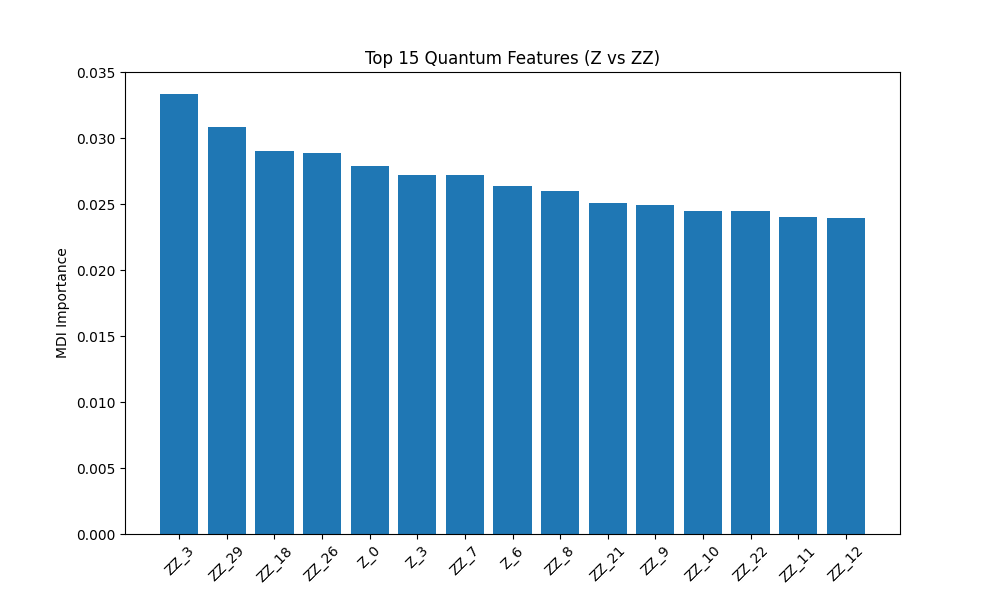
\includegraphics[width=0.7\textwidth]{images/aqcnn/feature_importance.png}
    \caption{Feature Importance Ranking using MDI. The top 15 most important individual features are almost exclusively $ZZ$ correlator pairs.}
    \label{fig:feature_importance}
\end{figure}

\section*{4. Experimental Plan \& Resource Estimation}
We utilize \textbf{Spatial Multiplexing} via Analog Hamiltonian Simulation (AHS) on the QuEra Aquila (256 qubits) to process patches in parallel. Due to the hardware's maximum Rabi frequency ($\Omega \approx 2.51 \text{ MHz}$), the minimum achievable Rydberg blockade radius ($R_b$) is $\approx 8.32 \mu m$.

To maximize spatial efficiency within the device's $75\mu m \times 76\mu m$ area, we encode a \textbf{King's graph} topology. By setting the intra-kernel lattice spacing to $4 \mu m$, the diagonal interactions ($5.65 \mu m$) naturally fall within the unavoidable $8.32 \mu m$ blockade. This compact topology, coupled with a $9 \mu m$ empty-space isolation boundary between grids, allows us to safely embed a maximum of 20 independent $3\times3$ kernels per task (180 total atoms). Quantum results will be \textbf{cached} for offline training.

\textbf{Workload:} (780 images $\times$ 81 patches) / 20 parallel patches = \textbf{3,159 tasks}.

\begin{table}[h]
    \centering
    \begin{tabular}{lrrr}
        \toprule
        Precision ($\epsilon$) & Shots per Task & Total Shots & \textbf{Estimated Cost (\$0.01/shot)} \\
        \midrule
        0.2 (20\% Error) & 25 & 78,975 & \textbf{\$789.75} \\
        0.1 (10\% Error) & 100 & 315,900 & \textbf{\$3,159.00} \\
        0.05 (5\% Error) & 400 & 1,263,600 & \textbf{\$12,636.00} \\
        \bottomrule
    \end{tabular}
\end{table}

\section*{5. Future Roadmap: Scaling to High-Resolution Imaging}
While this initial hardware phase focuses on $3\times3$ kernels, our architecture is built for scalability. Following the successful validation of these experiments, we will scale our framework to higher-resolution medical images using significantly larger quantum kernels (e.g., \textbf{4x4, 8x8, 16x16}). The 256-qubit array on QuEra Aquila provides the focal plane required to capture increasingly complex morphological features in large-scale colorectal cancer diagnostic datasets.

\begin{thebibliography}{9}
\bibitem{daqcnn2024}
Simen, A., Flores-Garrigos, C., Hegade, N. N., et al. (2024). \textit{Digital-analog quantum convolutional neural networks for image classification}. Phys. Rev. Research, 6(4), L042060.
\end{thebibliography}

\end{document}
